\documentclass{article}
\usepackage[utf8]{inputenc}
\usepackage{array}
\usepackage{multicol}
\usepackage{listings}
\usepackage{amssymb}
\usepackage{enumitem}
\usepackage{graphicx}
\usepackage{amsthm}
\usepackage{hyperref}
\usepackage{tikz}
\usepackage{amssymb}
\usepackage{amsmath}
\usepackage{mathtools}

\usetikzlibrary{automata,positioning}

\begin{document}

\title{Talen \& Automaten \\ Assignment 6}
\date{\today}
\author{Tony Lopar \enspace s1013792 \\TA: Nienke Wessel}
\maketitle

\section*{Exercise 1}
\begin{enumerate}[label= \alph*)]
  \item An automate that accepts $L_1$ is:
  \begin{center}
  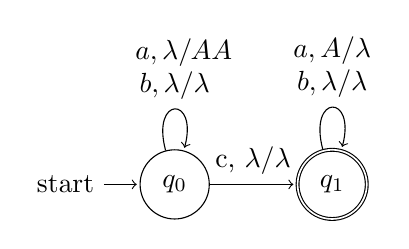
\begin{tikzpicture}[shorten >=1pt,node distance=2cm,on grid,auto]
     \node[state,initial] (q_0)   {$q_0$};
     \node[state, accepting] (q_1) [right=of q_0]  {$q_1$};
      \path[->]
      (q_0) edge [loop above]  node [text width=1cm,align=center] {$a, \lambda /AA$\\$b, \lambda / \lambda$} ()
            edge [left]  node [above] {c, $\lambda / \lambda$} (q_1)
      (q_1) edge [loop above]  node [text width=1cm,align=center] {$a, A / \lambda$\\$b, \lambda / \lambda$} ();
  \end{tikzpicture}
  \end{center}
  The PDA adds two A's on the stack for every `a' that's in w. The number of A's in v should be twice as much which is achieved by popping one A from the stack for every A.
  \item An automate that accepts $L_2$ is:
  \begin{center}
  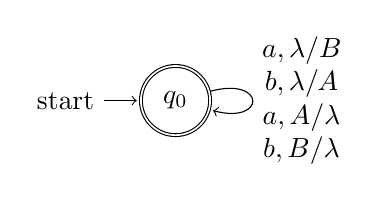
\begin{tikzpicture}[shorten >=1pt,node distance=2cm,on grid,auto]
     \node[state,initial, accepting] (q_0)   {$q_0$};
      \path[->]
      (q_0) edge [loop right]  node [text width=1cm,align=center] {$a, \lambda /B$\\$b, \lambda / A$\\$a, A / \lambda$\\$b, B / \lambda$} ();
  \end{tikzpicture}
  \end{center}
  The automate should have an equal number of A's and B's. This means that for every A in the word there should also be a B and vice versa. In this PDA in $q_0$ for every `a' a B is pushed to the stack and for every `b' an A. We may also pop elements from the stack in $q_0$. We may pop an A for `a' and a B for `b'. Since these elements are pushed on the stack while adding the other character, this makes sure that $|w|_a = |w|_b$ holds.

  We see that the word abba is accepted, because the accepting state is reached with an empty stack.
  \begin{align*}
    \langle q_0, abba, \lambda \rangle &\rightarrow \langle q_0, bba, B \rangle \\
    &\rightarrow \langle q_0, ba, \lambda \rangle \\
    &\rightarrow \langle q_0, a, A \rangle \\
    &\rightarrow \langle q_0, \lambda, \lambda \rangle
  \end{align*}

  We see that the word aa is not accepted, because after processing the word the stack contains BB.
  \begin{align*}
    \langle q_0, aa, \lambda \rangle &\rightarrow \langle q_0, a, B \rangle \\
    &\rightarrow \langle q_0, \lambda, BB \rangle
  \end{align*}
\end{enumerate}

\section*{Exercise 2}
% 2a -> L = {a, +, (, )} haakjes zitten in de grammar
\begin{enumerate}
  \item In order to turn this grammar into a PDA, we should first make it into the right form. It's currently not in the right form, since there is a + between the S in S and in F there is a ) after the S. A right-form grammar of this language could be:
  \begin{align*}
    S &\rightarrow F | SA \\
    F &\rightarrow a | (SC \\
    A &\rightarrow + S \\
    C &\rightarrow )
  \end{align*}
  The PDA of this language will be:
  \begin{center}
  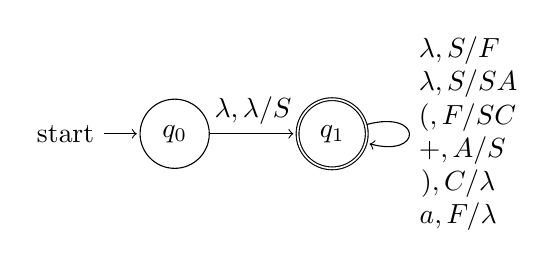
\begin{tikzpicture}[shorten >=1pt,node distance=2cm,on grid,auto]
     \node[state,initial] (q_0)   {$q_0$};
     \node[state, accepting] (q_1) [right=of q_0]  {$q_1$};
      \path[->]
      (q_0) edge [left]  node [above] {$\lambda, \lambda / S$} (q_1)
      (q_1) edge [loop right]  node [text width=1cm,align=center] {
            $\lambda, S / F$\\
            $\lambda, S / SA$\\
            $(, F / SC$\\
            $+, A / S$\\
            $), C / \lambda$\\
            $a, F / \lambda$
            } ();
  \end{tikzpicture}
  \end{center}
  \item The first step in converting the PDA to a context-free grammar is to split pushes and pops. This will give the following PDA:
  \begin{center}
  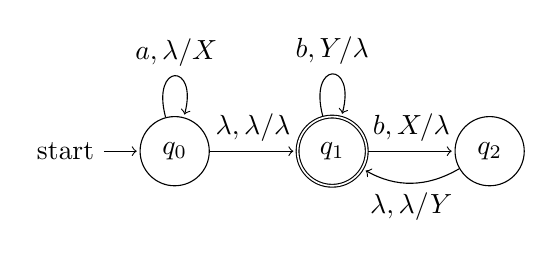
\begin{tikzpicture}[shorten >=1pt,node distance=2cm,on grid,auto]
     \node[state,initial] (q_0)   {$q_0$};
     \node[state, accepting] (q_1) [right=of q_0]  {$q_1$};
     \node[state] (q_2) [right=of q_1]  {$q_2$};
      \path[->]
      (q_0) edge [loop above]  node [text width=1cm,align=center] {$a, \lambda /X$} ()
            edge [left]  node [above] {$\lambda, \lambda / \lambda$} (q_1)
      (q_1) edge [loop above]  node [text width=1cm,align=center] {$b, Y / \lambda$} ()
            edge [left]  node [above] {$b, X / \lambda$} (q_2)
      (q_2) edge [bend left]  node [below] {$\lambda, \lambda / Y$} (q_1);
  \end{tikzpicture}
  \end{center}
  From this PDA we can derive the following context-free grammar for pairs of states. I left out the pairs that aren't used in the rest of the grammar.
  \begin{align*}
    S &\rightarrow (q_0, q_1) \\
    (q_0, q_1) &\rightarrow \lambda | a(q_0, q_1)b(q_1, q_2) \\
    (q_1, q_2) &\rightarrow \lambda(q_2, q_1)  \\
    (q_2, q_1) &\rightarrow b(q_1, q_1) \\
    (q_1, q_1) &\rightarrow \lambda
  \end{align*}

  We may derive the word `abb' in the following way:
  \begin{align*}
    S &\Rightarrow a(q_0, q_1)b(q_1, q_2) \Rightarrow ab(q_1, q_2) \Rightarrow ab(q_2, q_1) \Rightarrow abb(q_1, q_1) \Rightarrow abb
  \end{align*}

\end{enumerate}

\end{document}
